\section{Algoritma \& Flowchart}
Konsep Dasar, Simbol, Struktur, hingga Penerapannya.

\subsection{Pengertian Algoritma}
\textbf{Algoritma} adalah kumpulan langkah-langkah logis dan sistematis yang disusun secara berurutan untuk menyelesaikan suatu masalah atau mencapai tujuan tertentu. Setiap langkah dalam algoritma harus terdefinisi dengan jelas sehingga dapat dipahami dan dilaksanakan, baik oleh manusia maupun oleh komputer, tanpa menimbulkan makna ganda. 

Kata algoritma berasal dari kata "Algoritmi", yaitu nama latin dari matematikawan Persia bernama Abu Ja'far Muhammad Ibn Musa Al-Khawarizmi yang menjadi tokoh dasar lahirnya algoritma modern.

\textbf{Tujuan Algoritma:}
\begin{itemize}
    \item \textbf{Menyusun langkah penyelesaian masalah} secara terstruktur dan logis.
    \item \textbf{Mempermudah proses analisis dan perancangan program} sebelum implementasi penulisan kode.
    \item \textbf{Menjadi panduan universal} yang tidak bergantung pada sintaks bahasa pemrograman tertentu.
    \item \textbf{Meminimalkan kesalahan logika (\textit{logic error})} karena langkah dan kondisi dievaluasi secara jelas di awal.
\end{itemize}

\subsubsection{Ciri-ciri Algoritma yang Baik}
Menurut Donald E. Knuth, algoritma yang baik harus memenuhi kriteria berikut:
\begin{itemize}
    \item \textbf{Finiteness (Terbatas):} Harus berhenti setelah melakukan sejumlah langkah tertentu dan memiliki akhir yang jelas (tidak \textit{infinite loop}).
    \item \textbf{Definiteness (Jelas dan Tidak Ambigu):} Setiap langkah didefinisikan secara tegas tanpa penafsiran ganda.
    \item \textbf{Input:} Memiliki nol atau lebih data masukan sebelum atau selama proses.
    \item \textbf{Output:} Menghasilkan setidaknya satu keluaran dari hasil penyelesaian masalah.
    \item \textbf{Effectiveness (Efektif dan Efisien):} Langkahnya sederhana, wajar, dan hemat sumber daya.
\end{itemize}

\subsubsection{Cara Penyajian Algoritma}
\begin{description}
    \item[Kalimat Deskriptif:] Dituliskan dalam bentuk kalimat naratif menggunakan bahasa sehari-hari secara runtut. Mudah dipahami, namun kurang efektif untuk logika kompleks.
    \item[Pseudocode:] Penulisan menggunakan campuran bahasa manusia dan struktur mirip bahasa pemrograman. Lebih terstruktur dan mudah diterjemahkan ke dalam kode.
    \item[Flowchart:] Disajikan dalam bentuk diagram visual menggunakan simbol standar dan garis alir (\textit{flow line}). Sangat memudahkan pemahaman visual.
\end{description}

\subsection{Flowchart}
\textbf{Flowchart (diagram alir)} adalah representasi grafis dari suatu algoritma yang menggambarkan urutan proses dan keputusan logis menggunakan simbol-simbol standar (seperti kotak, oval, dan belah ketupat) yang dihubungkan dengan garis alir.

\subsubsection{Jenis-jenis Flowchart}
\begin{itemize}
    \item \textbf{Flowchart Sistem:} Menggambarkan alur kerja sistem secara keseluruhan (hardware, software, dan data).
    \item \textbf{Flowchart Dokumen:} Menggambarkan alur dokumen/formulir antar unit dalam organisasi.
    \item \textbf{Flowchart Skematik:} Mirip flowchart sistem namun dilengkapi dengan ilustrasi gambar fisik perangkat.
    \item \textbf{Flowchart Program:} Menggambarkan urutan instruksi program secara rinci (paling sering digunakan di pemrograman dasar).
    \item \textbf{Flowchart Proses:} Menggambarkan proses kerja dalam industri atau proses produksi.
\end{itemize}

\subsubsection{Struktur Dasar Algoritma/Flowchart}
Terdapat tiga struktur dasar untuk menyusun alur flowchart:

\textbf{1. Sequence (Runtutan)}

Instruksi dijalankan secara berurutan dari atas ke bawah, tanpa pengulangan atau percabangan.
\begin{center}
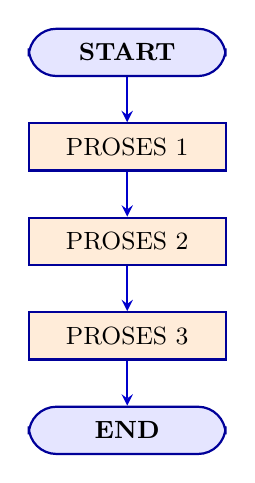
\begin{tikzpicture}[node distance=1.2cm, auto,
    layer/.style={draw=blue!60!black, thick, fill=blue!10, rounded corners=10pt, minimum width=2.5cm, minimum height=0.6cm, align=center, font=\bfseries\small},
    process/.style={draw=blue!60!black, thick, fill=orange!15, minimum width=2.5cm, minimum height=0.6cm, align=center, font=\small},
    arrow/.style={->, >=stealth, thick, color=blue!80!black}]
    
    \node (start) [layer] {START};
    \node (pro1) [process, below of=start] {PROSES 1};
    \node (pro2) [process, below of=pro1] {PROSES 2};
    \node (pro3) [process, below of=pro2] {PROSES 3};
    \node (end) [layer, below of=pro3] {END};
    
    \draw [arrow] (start) -- (pro1);
    \draw [arrow] (pro1) -- (pro2);
    \draw [arrow] (pro2) -- (pro3);
    \draw [arrow] (pro3) -- (end);
\end{tikzpicture}
\end{center}

\textbf{2. Selection (Percabangan/Branching)}

Program mengambil salah satu dari beberapa jalur proses berdasarkan suatu kondisi (\textit{IF-THEN-ELSE}).
\begin{center}
\begin{tikzpicture}[node distance=1.4cm, auto,
    layer/.style={draw=blue!60!black, thick, fill=blue!10, rounded corners=10pt, minimum width=2.5cm, minimum height=0.6cm, align=center, font=\bfseries\small},
    process/.style={draw=blue!60!black, thick, fill=orange!15, minimum width=2.5cm, minimum height=0.6cm, align=center, font=\small},
    decision/.style={diamond, aspect=1.6, draw=blue!60!black, thick, fill=green!15, minimum width=2.5cm, align=center, font=\small},
    arrow/.style={->, >=stealth, thick, color=blue!80!black}]
    
    \node (start) [layer] {START};
    \node (pro1) [process, below of=start] {PROSES 1};
    \node (dec) [decision, below of=pro1, yshift=-0.2cm] {KONDISI?};
    \node (pro2) [process, below left of=dec, xshift=-1.5cm, yshift=-0.8cm] {PROSES 2};
    \node (pro3) [process, below right of=dec, xshift=1.5cm, yshift=-0.8cm] {PROSES 3};
    \node (end) [layer, below of=dec, yshift=-2.2cm] {END};
    
    \draw [arrow] (start) -- (pro1);
    \draw [arrow] (pro1) -- (dec);
    \draw [arrow] (dec) -| node[anchor=south east, font=\footnotesize] {ya} (pro2);
    \draw [arrow] (dec) -| node[anchor=south west, font=\footnotesize] {tidak} (pro3);
    \draw [arrow] (pro2) |- (end);
    \draw [arrow] (pro3) |- (end);
\end{tikzpicture}
\end{center}

\textbf{3. Repetition (Perulangan/Looping)}

Satu atau beberapa instruksi dijalankan berulang kali selama suatu kondisi masih terpenuhi.
\begin{center}
\begin{tikzpicture}[node distance=1.4cm, auto,
    layer/.style={draw=blue!60!black, thick, fill=blue!10, rounded corners=10pt, minimum width=2.5cm, minimum height=0.6cm, align=center, font=\bfseries\small},
    process/.style={draw=blue!60!black, thick, fill=orange!15, minimum width=2.5cm, minimum height=0.6cm, align=center, font=\small},
    decision/.style={diamond, aspect=1.6, draw=blue!60!black, thick, fill=green!15, minimum width=2.5cm, align=center, font=\small},
    arrow/.style={->, >=stealth, thick, color=blue!80!black}]
    
    \node (start) [layer] {START};
    \node (pro1) [process, below of=start] {PROSES 1};
    \node (dec) [decision, below of=pro1, yshift=-0.2cm] {SYARAT?};
    \node (pro2) [process, below of=dec, yshift=-0.6cm] {PROSES 2};
    \node (end) [layer, below of=pro2] {END};
    
    \draw [arrow] (start) -- (pro1);
    \draw [arrow] (pro1) -- (dec);
    \draw [arrow] (dec) -- node[anchor=east, font=\footnotesize] {ya} (pro2);
    \draw [arrow] (pro2) -- (end);
    \draw [arrow] (dec) -- node[anchor=south, font=\footnotesize] {tidak} ++(2.5cm,0) |- (pro1);
\end{tikzpicture}
\end{center}

\subsubsection{Kaidah Membuat Flowchart}
\begin{enumerate}
    \item Digambar dari atas ke bawah dan dari kiri ke kanan secara konsisten.
    \item Hanya memiliki satu titik awal (\textit{start}) dan satu titik akhir (\textit{end}).
    \item Menggunakan simbol standar (ANSI/ISO) sesuai fungsinya.
    \item Gunakan kalimat aktif dan singkat pada keterangan langkah.
    \item Simbol \textit{decision} hanya boleh memiliki satu alur masuk, namun boleh memiliki beberapa alur keluar.
    \item Hindari alur saling silang; gunakan \textit{connector} jika diperlukan.
    \item Jaga jarak antar simbol secara proporsional agar mudah dibaca.
\end{enumerate}

\subsection{Perbedaan Algoritma dan Flowchart}
\begin{center}
    \begin{tabular}{l p{6cm} p{6cm}}
    \toprule
    \textbf{Aspek} & \textbf{Algoritma} & \textbf{Flowchart} \\ 
    \midrule
    \textbf{Sifat} & Abstrak dan fleksibel. & Konkret dan visual. \\ 
    \textbf{Penyajian} & Teks deskriptif atau \textit{pseudocode}. & Diagram dengan simbol standar. \\ 
    \textbf{Detail} & Bisa sangat umum maupun rinci. & Cenderung rinci karena tiap alur butuh simbol. \\ 
    \textbf{Keterbacaan} & Butuh penalaran bacaan teks logis. & Lebih cepat dipahami sekilas secara visual. \\ 
    \bottomrule
    \end{tabular}
\end{center}
